\documentclass{JNUexp}
\courseName{计算机图形学}
\expName{实验 2 线段和多边形的扫描转换}
\expDate{2017.11.12}
\className{计科1404}
\studentName{阎覃}
\studentId{1030414414}

\graphicspath{ {images/} }

\usepackage[hidelinks]{hyperref}
\usepackage{amsmath}
\begin{document} 

\section{实验内容}
\begin{itemize}
    \item 实现直线的DDA算法 
    \item 实现直线的中点算法
    \item 实现基于扫描线的多边形扫描转换算法
\end{itemize}

\section{实验步骤及运行情况}
%%%%%%%%%%%%%%%%%%%%%%%%%%%%%%%%%%%%%%%%%%%%%%%%%%%%%%%%%
%   1 实现直线的DDA算法
%%%%%%%%%%%%%%%%%%%%%%%%%%%%%%%%%%%%%%%%%%%%%%%%%%%%%%%%%
\begin{problem}
    实现直线的DDA算法 
\end{problem}
\begin{answer}
    数值微分法(DDA法)根据直线的微分方程来绘制直线,它是最简单的一种画线方法。
    若一条直线的起点为$\left(x_1,y_1\right)$,终点为$\left(x_2,y_2\right)$,令
    \begin{align*}
        \Delta x &= x_2-x_1 \\
        \Delta y &= y_2-y_1 \\
        \Delta m &= max(\left|\Delta x \right|,\left| \Delta y\right|)
    \end{align*}
    则可以得到递推公式为
    \begin{align}
        \Delta x_{i+1} &= x_i + \frac{\Delta x}{\Delta m}\\
        \Delta y_{i+1} &= y_i + \frac{\Delta y}{\Delta m}
    \end{align}
    因此,直线的DDA算法程序为
    \lstinputlisting[language={[11]C++},title=Entities/LineDDA2D.cpp]{../src/Entities/LineDDA2D.cpp}
    本程序参考书上代码P42。
\end{answer}
\begin{image}
    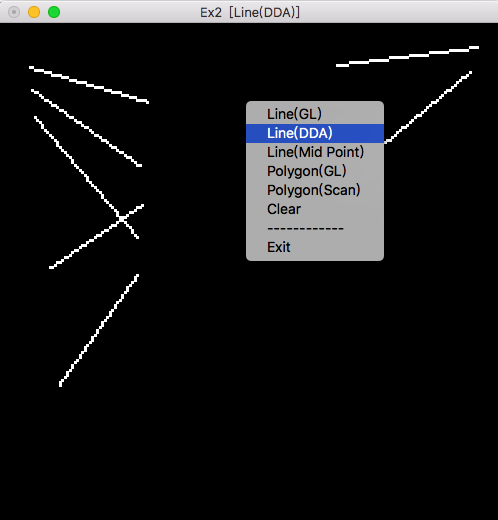
\includegraphics[width=0.7\textwidth]{1}
\end{image}
%%%%%%%%%%%%%%%%%%%%%%%%%%%%%%%%%%%%%%%%%%%%%%%%%%%%%%%%%
%   2 实现直线的中点算法
%%%%%%%%%%%%%%%%%%%%%%%%%%%%%%%%%%%%%%%%%%%%%%%%%%%%%%%%%
\begin{problem}
    实现直线的中点算法
\end{problem}
\begin{answer}
    若一条直线的起点为$\left(x_0,y_0\right)$,终点为$\left(x_1,y_1\right)$,直线方程为
    \begin{equation*}
        F(x,y) = ax+by+c=0
    \end{equation*}
    其中,$a=y_0-y_1$,$b=x_1-y_0$,$c=x_0y_1-x_1y_0$。\\
    若当前的点为$\left(x_p,y_p\right)$,则可以带入下一中点,构造判别式:
    \begin{equation}
        \begin{split}
            d &= F(x_p+1,y_p+0.5) \\
              &= a(x_p+1)+b(y_p+0.5)+c
        \end{split}
    \end{equation}
    $d<0$时取右上方点,$d\ge 0$取右方点。\\
    为了提高效率,可以采用增量算法。\\
    当斜率为正:\\
    当$d\ge 0$时,$d'=d+a$ \\
    当$d < 0$时,$d'=d+a+b$ \\
    当斜率为负:\\
    当$d\ge 0$时,$d'=d-a$ \\
    当$d < 0$时,$d'=d-a+b$ \\

    因此,直线的中点算法程序为
    \lstinputlisting[language={[11]C++},title=Entities/LineMidP2D.cpp]{../src/Entities/LineMidP2D.cpp}
    本程序参考书上代码P49,P50。
\end{answer}
\begin{image}
    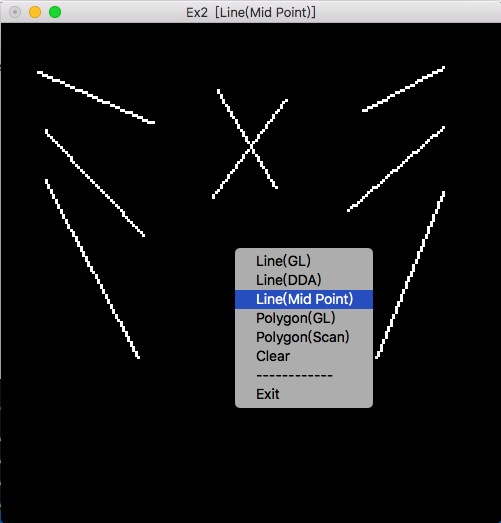
\includegraphics[width=0.7\textwidth]{2}
\end{image}
%%%%%%%%%%%%%%%%%%%%%%%%%%%%%%%%%%%%%%%%%%%%%%%%%%%%%%%%%
%   3 实现基于扫描线的多边形扫描转换算法
%%%%%%%%%%%%%%%%%%%%%%%%%%%%%%%%%%%%%%%%%%%%%%%%%%%%%%%%%
\begin{problem}
    实现基于扫描线的多边形扫描转换算法
\end{problem}
\begin{answer}
    定义边节点:
    \begin{lstlisting}[language={[11]C++}]
class Edge {
public:
    int ymax;
    float x;
    float dx;
    Edge *next;
};
    \end{lstlisting}
    其中,ymax为该边最大的y坐标,x为y值最小的端点的x坐标,dx为斜率。\\
    定义一个边表数组ET,存放所有的边。数组大小为扫描线的数目。定义一个链表AET,即活动边表,表示正在处理的扫描线。\\
    具体的算法如下:
    \begin{enumerate}
        \item 初始化ET,将各边按照该边最小的y坐标存放至数组内对应位置。
        \item 初始化AET为空链表。
        \item 扫描线从下向上扫描,y从0增加至最大值,每次加1。
        \begin{enumerate}
            \item 取出ET中当前扫描线的所有边并按x递增的顺序加入AET。
            \item AET中的边两两配对并填色。
            \item 删除AET中满足y=ymax的边。
            \item 更新AET中边的x值,进入下一循环
        \end{enumerate}
    \end{enumerate}

    对于本程序坐标系的范围是-100至100,所以要对所有的y值进行偏移以便消去负数放入数组中。
    \lstinputlisting[language={[11]C++},title=Entities/PolygonScan2D.cpp]{../src/Entities/PolygonScan2D.cpp}

\end{answer}
\begin{image}
    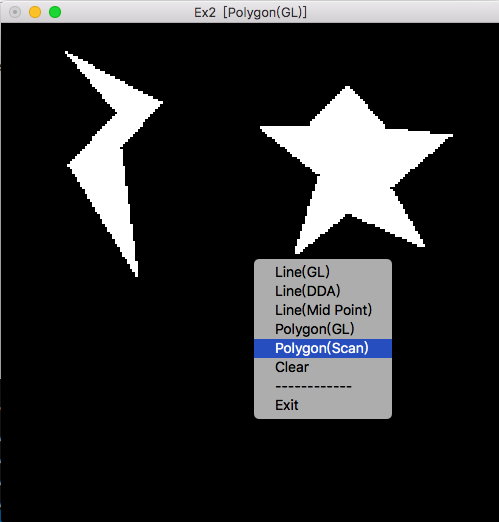
\includegraphics[width=0.7\textwidth]{3}
\end{image}
\newpage
\section{实验体会}
前两个直线的算法非常简单,并且书上提供了代码,很快就可以做出来。然而第三个书并没有提供代码,
只有文字说明算法的步骤。但是由于本人理解能力有限,还是没能看懂。所以我在网上搜索了一下,发现
\url{http://www.twinklingstar.cn/2013/325/region-polygon-fill-scan-line/}这篇
文章讲的比较详细清楚。之后又参照了相关代码,完成了本次作业。

\vfill

实验报告采用 \LaTeX 排版,完整代码托管至GitHub:\\
\url{https://github.com/Ethan-yt/JNU-CG-exp}

\end{document}